\documentclass[10pt,twocolumn,letterpaper]{article}

\usepackage{cvpr}
\usepackage{times}
\usepackage{epsfig}
\usepackage{graphicx}
\usepackage{amsmath}
\usepackage{amssymb}

% Include other packages here, before hyperref.

% If you comment hyperref and then uncomment it, you should delete
% egpaper.aux before re-running latex.  (Or just hit 'q' on the first latex
% run, let it finish, and you should be clear).
\usepackage[pagebackref=true,breaklinks=true,letterpaper=true,colorlinks,bookmarks=false]{hyperref}

% \cvprfinalcopy % *** Uncomment this line for the final submission

\def\cvprPaperID{****} % *** Enter the CVPR Paper ID here
\def\httilde{\mbox{\tt\raisebox{-.5ex}{\symbol{126}}}}

% Pages are numbered in submission mode, and unnumbered in camera-ready
\ifcvprfinal\pagestyle{empty}\fi
\begin{document}

%%%%%%%%% TITLE
\title{UFo - Coupling Uncertain Active Constellation Models with \\
Cascaded Forest Predictors for Sematic Segmentation}

\author{First Author\\
Institution1\\
Institution1 address\\
{\tt\small firstauthor@i1.org}
% For a paper whose authors are all at the same institution,
% omit the following lines up until the closing ``}''.
% Additional authors and addresses can be added with ``\and'',
% just like the second author.
% To save space, use either the email address or home page, not both
\and
Second Author\\
Institution2\\
First line of institution2 address\\
{\tt\small secondauthor@i2.org}
}

\maketitle
%\thispagestyle{empty}

%%%%%%%%% ABSTRACT
\begin{abstract}
We consider the task of model-based semantic segmentation. The model is described by a constellation model of parts that are represented by active shape- and appearance models. We term this an active constellation model. As a running example we utilize a 21-part, chain-based spine model of a zebra fish observed in microscopic images. The prevailing approach to solve this task is to first generate pixel-independent features for each part, e.g.\ via a cascaded decision forest predictor, which are then fed into an MRF-based model-fitting objective to infer the optimal MAP solution of the constellation model. Our key contribution is to abandon this static, two-stage approach and mix feature generation and model-based inference in a new, more flexible, way. In particular we interleave the cascaded forest predictors with inference steps for the model-fitting. A key finding is that “uncertain” model-outputs at intermediate stages of the cascade, in the form of part-based marginals, are essential for best performance. This is because, on one hand the semantic segmentation is guided by the model, and on the other hand correct solutions, which are different to intermediate MAP solution, can still be found. We validate our findings with an in-depth study of alternative inference steps, including popular geodesic smoothing as well as MAP inference. %, and alternative output generation steps, including max-marginals. 
We believe that our findings are not only relevant for other types of constellation models but, more generally, for the recent trend of combing deep learning models with physically-motivated structured models. 
\end{abstract}

\begin{figure*}[t]
\begin{center}
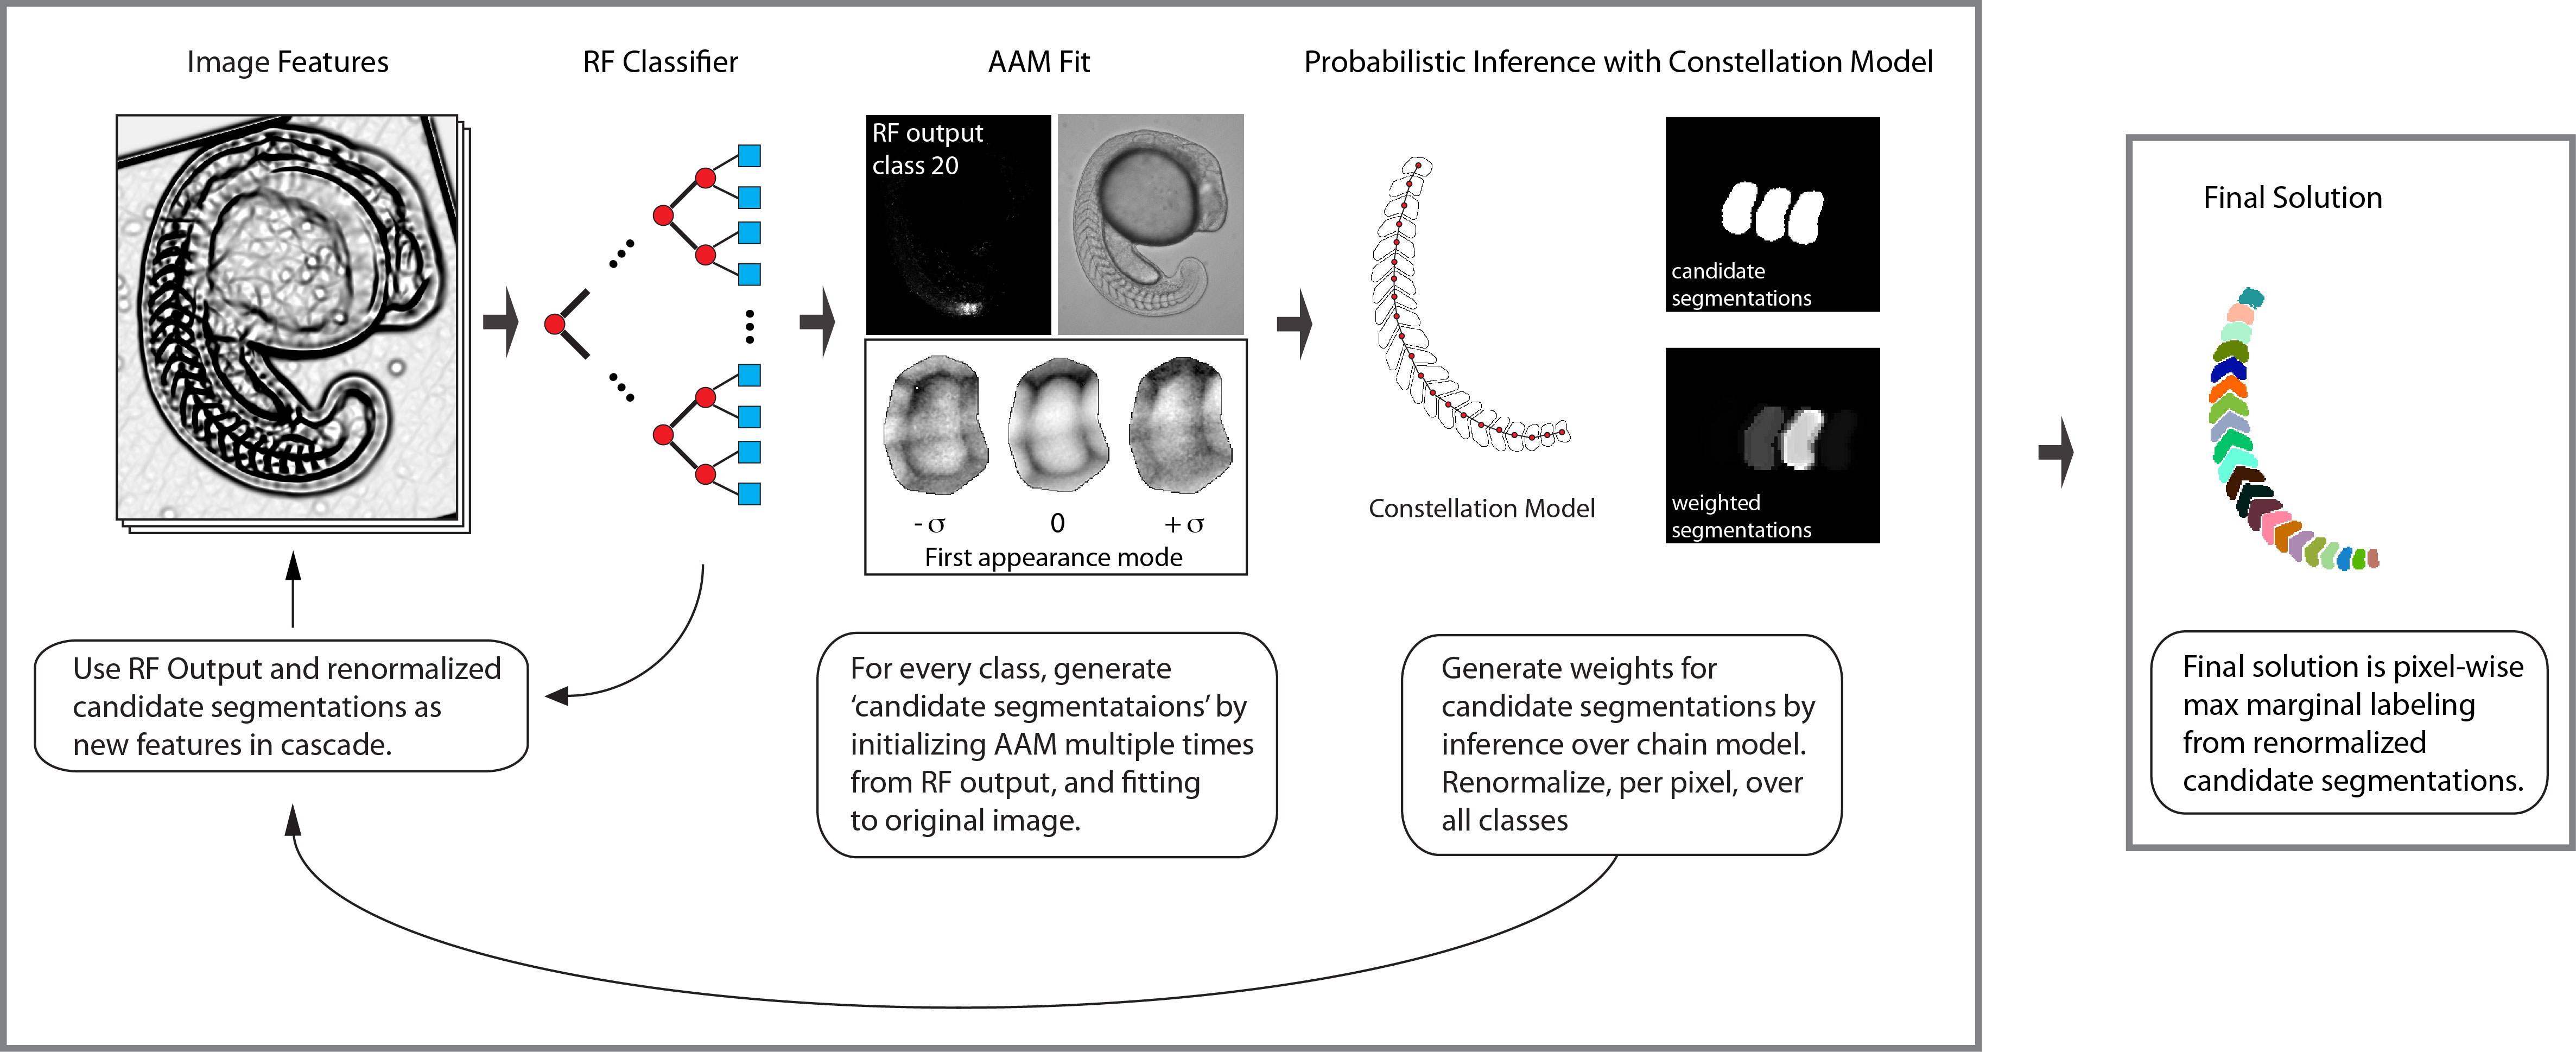
\includegraphics[width=\textwidth]{pipelineBIG.jpg} %&[trim=0cm 2cm 0cm 1cm,height=0.2\textheight]
\caption{Pipeline.}
\label{fig:pipeline}
\end{center}
\end{figure*}


\section{Introduction}
Many tasks in computer vision have as input an image and as output a dense labeling, where each pixel is assigned one out of many pre-defined classes. An example is a sematic segmentation of a person in an image, where each pixel is assigned a label such as “background”, “left leg”, or “head”. 
%
So-called structured models, such as a Conditional Random Field (CRFs), are often used for semantic segmentation. 
Depending on the prior knowledge about the task at hand, the underlying graph may be a (super-)pixel grid, or a graphical constellation model that captures relative locations of multiple parts of an object. 
%
Furthermore, knowledge about distinct shapes of sought objects or parts of objects is often captured by means of statistical shape and appearance models. 

All these models commonly capture the task of semantic segmentation via an objective function that is composed of a data term and a prior. 
%
The data term, referred to as "`features"', is derived from the image at hand, yielding pixel-wise distributions over class labels. The prior is enforced subsequently. 
%
% from image data that gives for each individual pixel a distribution over class labels. These class-label distributions define the unary potentials in the CRF
%
Classical approaches employ pixel-wise classifiers combined with MAP inference on a (super-)pixel grid graph for segmentation [], or with MAP inference on a graphical constellation model for the localization of object parts [Glocker, Dental,Worm, SeifertAbdominal].  
%
This modelling framework is however very static, as it separates feature generation and inference (i.e.\ "`model fitting"'). 

A recent trend in computer vision is to learn deep, \emph{cascaded} models for feature generation, such as CNNs~\cite{NIPS2012_4824} (see also e.g.\ \cite{funke2014candidate}) and Auto-Context Models~\cite{AutoContext2008} (see also e.g.\ \cite{PoseMachinesECCV2014}). 
%
These models play the role of learning a complex non-linear mapping from images to features which are relevant for the task at hand. 
%
Beyond cascading, it has been shown that better features can be generated by \emph{interleaving} feature generation with MAP inference in pixel-grid structured models~\cite{DTF,RTF,UweCVPR2013} 
%
or model agnostic smoothing smoothing~\cite{GeoForests2013}.\footnote{Note that this is different from the classical "`hierarchical"' approach that, purely for the sake of run-time, performs feature generation and inference multiple times on different scales (see e.g.\ \cite{CootesECCV2012RRFandSSM,CootesFemurTMI2013} [check!]).}

In this work we take the idea of interleaving feature generation and inference a step further: 
%
Instead of interleaving feature generation with a pixel-level structured model or model-agnostic smoothing, we interleave with a global, generative \emph{active constellation model}. By this term we refer to a graphical constellation model, where the individual object parts are captured by \emph{active appearance models}~\cite{CootesAAM2001}. 
%
We suggest a cascaded pipeline, as illustrated in Figure~\ref{fig:pipeline}. 
% 
The most important aspect of this cascade is the question of what to infer from the constellation at intermediate stages of the cascade. 
%
"`Model based"' options are marginals or MAP solution of the MRF-based constellation model. A model-agnostic, yet "`image-aware"' alternative is geodesic smoothing~\cite{GeoForests2013}. 
%
One of the main aspects of this work is to study the trade-offs that come with these options. 

We show that soft marginals are a clear winner for an application concerned with semantic segmentation of many self-similar structures, namely vertebrae in spines of zebra-fish embryos. 
%
(These vertebrae are called "`somites"'.) 
%
The reason that \emph{uncertainy is beneficial} is that individual somites are highly ambiguous with respect to shape and appearance, hence only the relative spatial arrangement can disambiguate this situation. 
%
Related work has tackled semantic segmentation of vertebrae (in CT scans of humans) via the classical "`feature generation followed by MAP in a constellation model"' approach~\cite{Glocker2013}.
%
We show that marginals instead of MAP helps to not commit to a wrong solution in the early stages of a cascade, and leads to a major increase in resulting segmentation accuracy. 

Closely related to the presented work are 
(1) Auto Context~\cite{AutoContext2008}, but they do not perform any smoothing in between levels of the cascade. 
(2) Geodesic Forests~\cite{GeoForests2013}, but they do not use a generative structured model for smoothing. 
(3) Cascaded classifiers interleaved with MAP inference~\cite{}, but they do not use a global generative model and do not explore marginals for inference. 
(4) Constellation models for vertebrae and other self-similar object segmentation~\cite{Glocker2012,Glocker2013,Klinder2009471,TeethMICCAI2012,WormMiccai2014} but they do not run a cascade. 

To summarize, we claim the following three {\bf contributions}:
\begin{itemize}
\item In the field of model-based semantic segmentation we are the first to interleave feature generation and model-based inference. We show that this boost performance considerably, compared to not cascading. 
% Note, related hierachical appraoches~\cite{CootesECCV2012RRFandSSM,CootesFemurTMI2013} focus on speed not quality that comes form feature generation. 
\item We show, for the first time, that probabilistic inference gives a major (6\%) boost in performance in cascaded MRF-Forest-based models. This is compared to standard MAP inference (as e.g.\ in \cite{Glocker2013,SeifertAnatomicalSPIE2009,TeethMICCAI2012}) and model-agnostic geodesic smoothing~\cite{GeoForests2013}. 
\item We are the first to tackle spine detection in zebra fish, where we achieve an overall average Dice score of 82\%.
\end{itemize}



ToDo: Work in or leave out:
%
Another way to look at this is that we want to mix discriminative (discr) and generative models (gen), in a smart way.  E.g., The discr model initializes the gen model in the right search space, the gen model then refines this initialization.  This process is iterated while simultaneously increasing the "confidence" in the discr model output. 
%
Additional Literature: 
%
Deformable Templates Guided Discriminative Models for Robust 3D Brain MRI Segmentation.~\cite{BrainSeg2013}  Liu et al.  2013: Uses generative model to "refine" features in a cascaded discriminative classifier.
%
Uwe's hint \cite{Denzler2012}: As Time Goes by -- Anytime Semantic Segmentation with Iterative Context Forests

\emph{Related work on Constellation models and Forests: }
%
Spine: Glocker~\cite{Glocker2013}; 
%
Body parts: Auto Context~\cite{AutoContext2008}, "`Pose Machines"' ECCV 2014~\cite{PoseMachinesECCV2014}; 
% 
Abdominal images: GeoF~\cite{GeoForests2013}, and GeoF at IPMI 2011~\cite{CriminisiAbdominalIPMI2011}: "'Entangled Decision Forests and their Application for Semantic Segmentation of CT Images"'. Seifert SPIE: Marginal space learning classifier plus MRF~\cite{SeifertAnatomicalSPIE2009} 

\section{Background}

\paragraph{Random Forests and Cascading. }
We assume that the reader is familiar with the general concept of Random Forests (RF)~\cite{BreimanRF}. 
%
In the Auto Context approach~\cite{AutoContext2008}, the probability maps yielded by a random forest are fed as features into subsequent random forests, yielding a cascade of forests.  
%
Interleaved inference/smoothing operates on these probability maps, and feeds ``smoothed'' versions of them into the next forest~\cite{DTF,RTF,UweCVPR2013,GeoForests2013}. 
%



\paragraph{AAM. Dave, please work on this. Should be 0.5p max. Terminology as in Cootes papers.}
Active appearance models (AAMs)~\cite{CootesAAM2001} are linear, generative, parametric models of shape and appearance that are learned (PCA) from training data.  Fitting an AAM is a non-linear optimisation problem, that is done via incremental updates to fitting parameters.  Importantly, AAMs can be easily extended to include priors on the model parameters (see also~\cite{BakerAAM2004}).  

Shape Model:

\[s = s_0 + \sum_{i=1}^n p_i s_i\]

where s is a vector of x,y coordinates of the landmarks that define the shape.  From PCA, $s_0$ is the mean shape, and $s_i$ are n eigenvectors corresponding to the n largest eigenvalues.  Not shown here is that the training data is first noramlised using a Procrustes analysis using a global shape normalising transformation (in our case, a similarity transform) to avoid modeling this variation in the linear model.

Appearance Model:

\[A(x) = A_0(x) + \sum_{i=1}^m \lambda_i A_i(x)\]

Analogous to shape model. $A_0$ and $A_i$ are computed from PCA on a set of \emph{shape normalised} training images, which have been warped onto the base-mesh $s_0$.  Shape normalizing is a key benefit of AAMs (compared to e.g. Eigen-faces), and leads to more compressed PCA representation.

To create a model instance, create an image A(x) (defined by $\lambda$) on the base-mesh, and then warp it to s (defined by p).  Warping is done using a thin-plate spline, parameterized by the set of landmarks, $s_0$ and s.  This defines the unique warp parameterised by p, called W(x;p).

Fitting criteria:

\[Error = A_0(x) + \sum_{i=1}^m \lambda_i A_i(x) - I(N(W(x;p);q)) \]

where N(x;q) is the similarity transform, parameterized by q, and the cost is typically the sum of squared errors over the shape normalized patch.

\[Cost = \sum_{x \epsilon s_0} [Error]^2 \]

Final note, the most efficient fitting routine [] actually "projects out" the appearance variation (from the Error image), and simply solves for the parameters of the transformation: p,q.  If you keep one shape parameter (n=1), this leads to a 5 parameter model.


One can add priors on the model parameters, as follows:

\[ \sum_{x \epsilon s_0} [A(x) - I(N(W(x;p);q)]^2 + \sum_{i=1}^K F_i^2(p,q) \]

If $F_i(p,q)$ is quadratic, this can be interpreted in the Bayesian framework as Gaussian Regularization.  There's also a clear way to "ramp" the importance of the priors as:

\[ F_i^2(p,q) = r[(p-p_0)^2+(q-q_0)^2]) \]

where r is the parameter that captures how much we trust the discr model output (this could be learned). 

Note, adding priors doesn't slow down the code too much.  You can still use the same fitting algorithm, there's just some extra computation in each loop.

\emph{Related work on SSMs and Random Forests: }



\section{Method}
Given an image as input, we seek a pixel-wise multi-class labelling as output, i.e.\ a \emph{semantic segmentation}. 
%
We assume that a model of the spatial relation of classes can be learned, i.e.\ a \emph{constellation model}. This is the case for many applications, as e.g.\ body part segmentation~\cite{PoseMachines2014}, organ segmentation in abdominal images~\cite{SeifertAnatomicalSPIE2009}, spine segmentation~\cite{Glocker2012,Glocker2013}, etc. 
%

We propose the following pipeline for \emph{model-based semantic segmentation}, as layed out in Figure~\ref{fig:pipeline}: 
%
First, we generate probability maps for each class with a random forest (RF) classifier.
%
Second, we generate many \emph{part proposals} for each class, with the help of Active Appearance models (cf.\ Sec.\ \ref{subsec:hyps}). 
Each part proposal is a binary segmentation of the respective class. It serves as a ``segmentation hypothesis''. 
%
Third, we perform probabilistic inference in a constellation model to weigh part proposals (cf.\ Sec.\ \ref{subsec:weightsAndFusion}), and effectively ``smooth'' the probability maps generated by the RF classifier.  
%
Fourth, we feed the resulting ``smoothed'' probability maps, together with the original probability maps as well as all image features used as input to the previous RF, into a next RF classifier. 
%
To generate a resulting labeling per pixel from the last RF output in the cascade, one can take the class with maximum probability according to either the RF probability maps, or the respective ``smoothed'' versions. 


\subsection{Generating Part Proposals}
\label{subsec:hyps}
%
Given an RF-generated probability map of a class, we
First compute its centroid via the mean shift algorithm. 
%
Second, we fit an average constellation model (i.e.\ a static constellation of landmarks) to these centroids to yield an optimal global similarity transform w.r.t.\ the sum of squared landmark distances. In our application, this is sufficient to define an approximate orientation of the part. 
%
Third, we sample a number of candidate locations around the centroids of the RF-generated probability maps to get sets of location initializations for the respective classes. 
%
Fourth, we fit a class specific active appearance model (AAM) to the image, multiple times, starting at the initial locations computed in the previous step. 
%
Each AAM fit results in a binary segmentation, together with a cost for the fit (cf.\ Eq.\ \eqref{}). 
%
These binary segmentations serve as part proposals, i.e.\ segmentation hypotheses for their respective classes. 

\subsection{Weighting and Fusing Part Proposals}
\label{subsec:weightsAndFusion}

Pairwise MRF.

Nodes: $c\in \{1..n_C\}=:C$=Classes

Labels: $l\in \{1..n_L\}=:L$=Part Proposals. (Here: Same number $n_L$ for all classes.)

Unaries: $\phi_c(l)$=AAMFit and integrated RF output

Binaries: $\psi_{c,b}(l,k)$ =Learnt from Training Data

By the above method, a number of model instances are initialized and fit, for each class.  Each model instance has a cost associated with its fit.  Use these costs as unaries in a Markov Chain Model.  The pair-wise energy comes from statistics on the relative position of neighboring segments in the training data.  This is exactly what Glocker did already; however, we do probabilistic inference (rather than MAP inference) and keep all the marginals.

Recall, since we initialized many AAMS for fitting, and did probabilistic inference over all of these solutions, we have multiple masks each with its own probability.  For each class c, compute a weighted average:

\[ P_c(x,y) = \frac{1}{Z(x,y)} \cdot \sum_{l\in L} p_c(l)\cdot H_{l,c}(x,y) \]

where there are L model instances initialized (for ease of notation, same number for all classes), $H_{l,c}$ is the binary mask that represents the $l$-th proposal for class $c$, and $p_c(l)$ is the marginal probability of model instance l being the true segmentation of class c, as obtained by probabilistic inference, and $Z(x,y)$ serves for pixel-wise re-normalization. I.e., $Z(x,y)=\sum_{c\in C}\sum_{l\in L} p_c(l)\times H_{l,c}(x,y)$.

We call $P_c$ the \emph{smoothed probability map} for class $c$. 

\subsection{Parameters}
... to be put into respective equations spread everywhere...
\begin{itemize}
\item n: \# of shape modes
\item m: \# of appearance modes
\item r: trust in discr output
\item S: \# of model instances that are initialized for fitting
\item g: \# of grad descent steps
\end{itemize}

\section{Results}
Approach: Cascade interleaved with "`smoothing"'. 

In our approach we employ Classification Forests, where features stem from a standard filter bank [Weka], together with offset and difference features. 
%

Evaluation: Different kinds of "`smoothing"', each with different kinds of outputs.

Dataset: 32 light microscopic images of developing zebra-fish. Task: Semantic segmentation of 21 somites (i.e.\ developing vertebrae). 
%
We perform a two-fold cross validation. We explore four different approaches. 

\begin{figure}[t]
\begin{center}
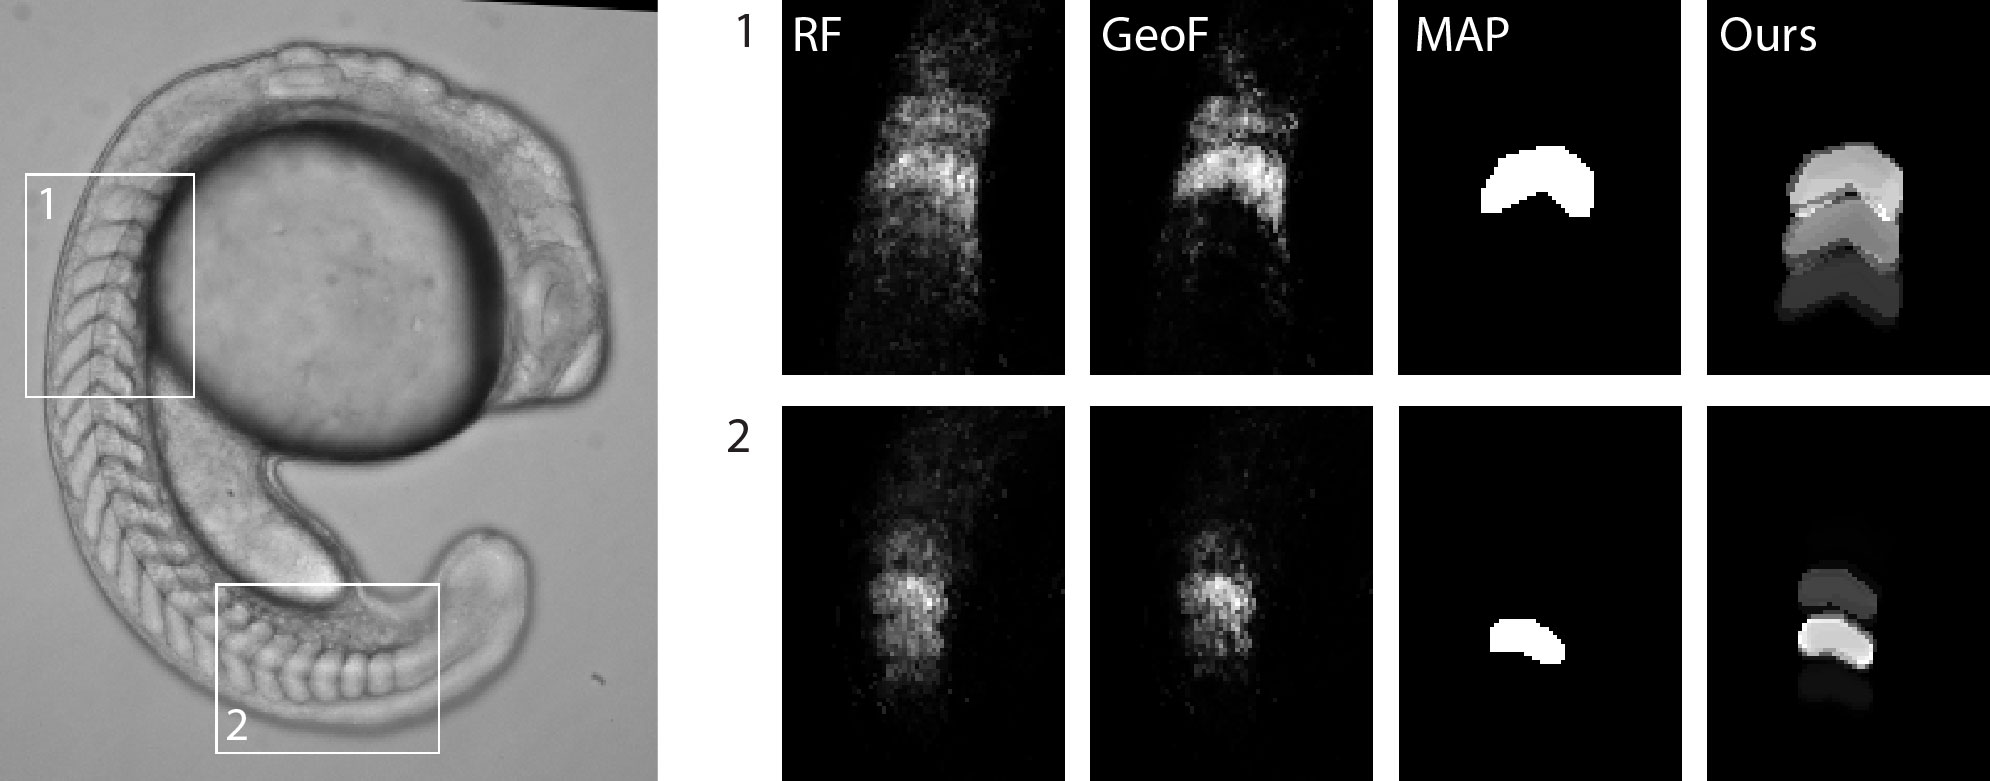
\includegraphics[width=\columnwidth]{smoothing.jpg} %&[trim=0cm 2cm 0cm 1cm,height=0.2\textheight]
\caption{In our evaluation we interleave different types of inference/smoothing into our cascaded random forest pipeline for semantic segmentation of somites (i.e.\ vertebrae) in zebra-fish embryos. 
%
The Figure shows examples of the types of inference/smoothing we evaluate. 
Left: Exemplary zebra-fish embryo. Boxes (1,2): Exemplary somites. Right: Close-ups on probability maps of the respective class labels. Note that close-ups on (2) are rotated by 90 degrees. 
%
Four versions of smoothing/inference: (RF) random forest probability map; (GeoF) smoothed by geodesic smoothing\cite{GeoF2013}; (MAP) "`smoothed"' by MAP inference in our constellation model, yielding a binary "`probability map"'; 
%
(MM) "`smoothed"' by our proposed approach, i.e.\ probabilistic inference in our constellation model.  }
\label{fig:smoothing}
\end{center}
\end{figure}
%
Figure \ref{fig:smoothing} show the different types for inference/smoothing we evaluate. 

\paragraph{Ours. }
AAM with probabilistic inference 

\paragraph{Auto Context. }

\paragraph{GeoF. }
The simplest way to generate a smoothed RF Output is to re-use the Geodesic smoothing idea from Criminisi.  Let:

\[ Q(x; M, \nabla I) = \min_{x'} (\delta (x,x') + \nu M) \]

and $\nu$ is some free parameter.  Note, x and x' are two points in the image. $M(x') = 1 - p(c|v(x'))$, where v(x') is the feature vector at pixel x'.  Then the smoothed RF output is calculated as:

\[ g(c|v(x)) = \frac{1}{Z} p(c|v(x)) e^{\frac{-Q(x;p(c|v(\Omega)),\nabla J)^2}{\sigma ^2}} \]

This accomplishes smoothing in quite an indirect way, as a competition between different possible class labels for a given pixel, mediated by the normalization Z.  

\paragraph{MAP Inference. }

\begin{figure}[t]
\begin{center}
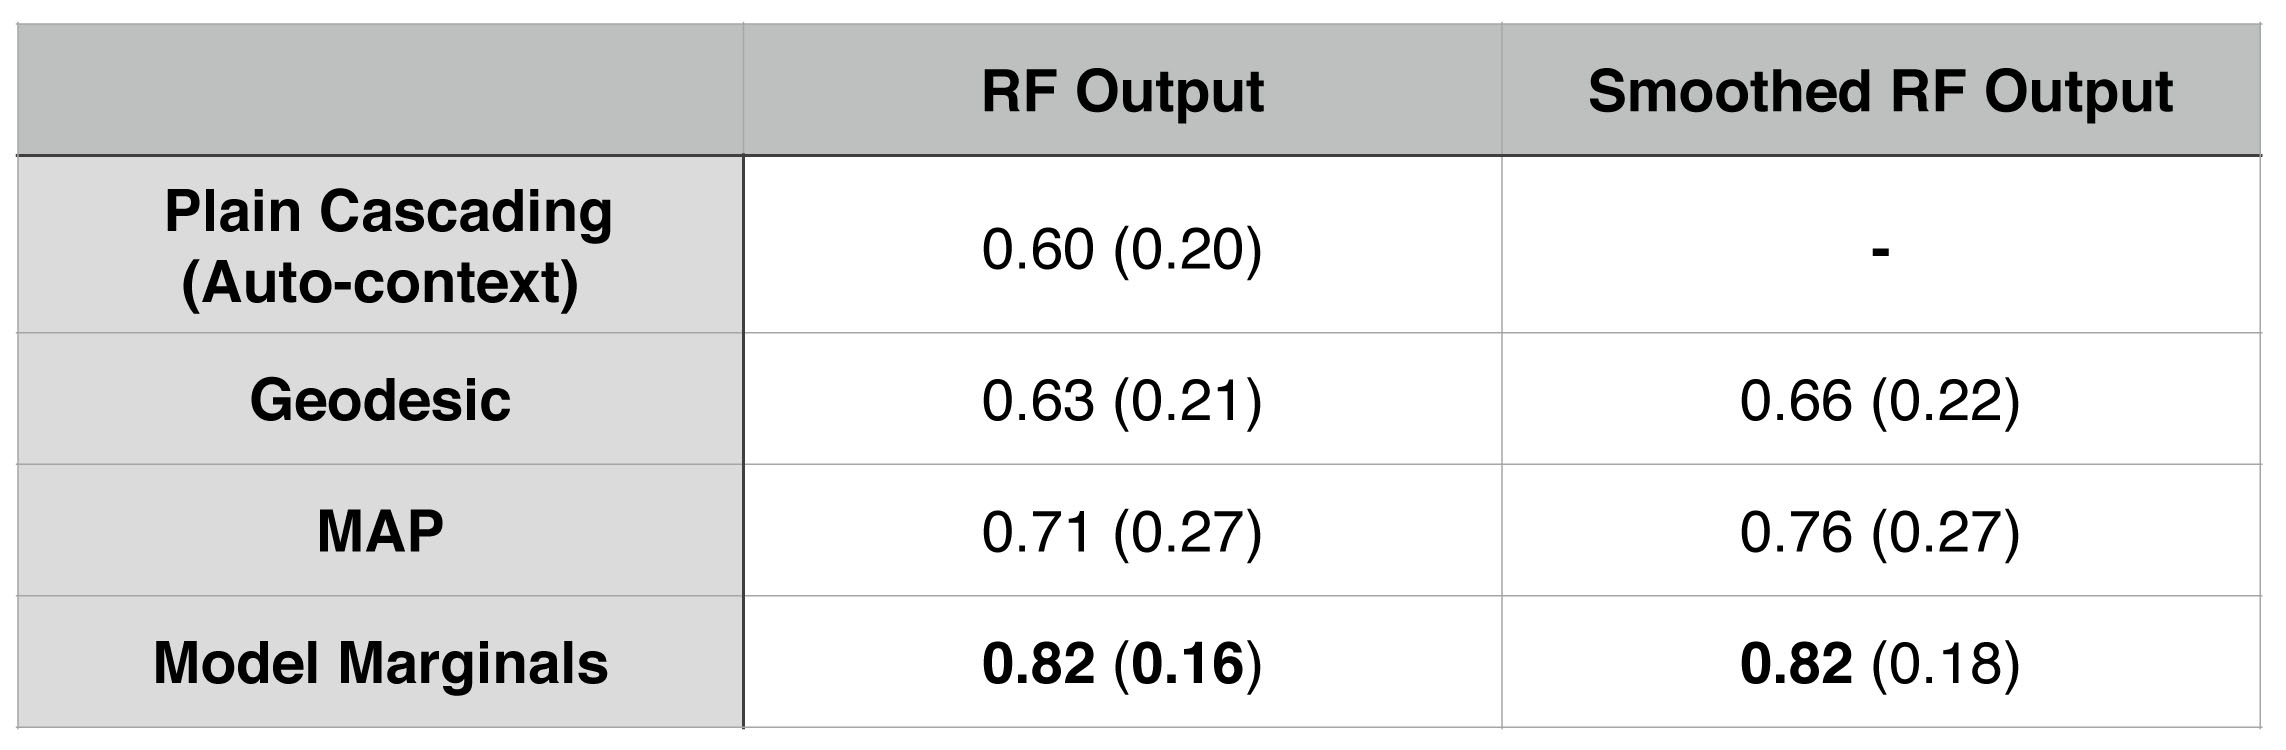
\includegraphics[width=\columnwidth]{TableDiceScores_2columns_noGeoF2.jpg} %&[trim=0cm 2cm 0cm 1cm,height=0.2\textheight]
\caption{Evaluation on 32 datasets. Dice Scores on all 21 Somites: Mean and standard deviation (in brackets).}
\label{tab:results}
\end{center}
\end{figure}

\begin{figure}[tb]
\centering
\small
\begin{center}
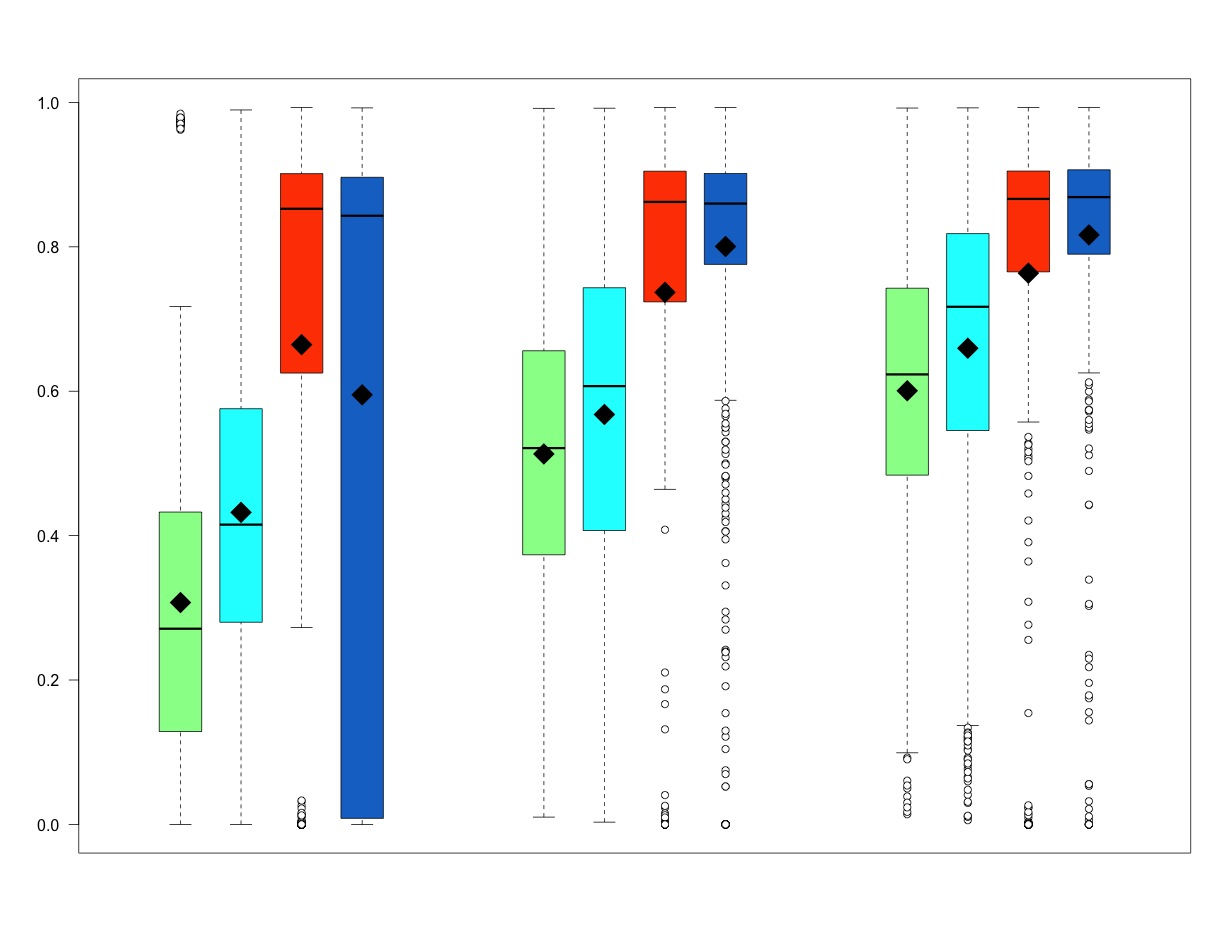
\includegraphics[width=\columnwidth]{Cascade.jpeg} %&[trim=0cm 2cm 0cm 1cm,height=0.2\textheight]
\end{center}
\label{fig:boxplots}
% \vspace{-2mm}
\caption{3 level cascade. Segmentation accuracy of 4 methods after each level: RF output (green), GeoF (cyan), MAP (red), Ours (blue). For every method at every level, Dice scores of 21 somites in 32 images, i.e.\ 672 scores, are visualized as a \emph{box plot}~\cite{chambers1983graphical}. A colored box spans from lower to upper quartile, i.e.\ the inter-quartile range. I.e.\ 50\% of the data points lie within the box. The horizontal bar within the box depicts the median. The black diamond depicts the mean. Whiskers depict the outlier-free data range. Circles depict outliers. Outliers are defined as data points beyond median $\pm$ 2 inter-quartile ranges. }
\end{figure}

\section{Discussion}
Ours is the best :)

\paragraph{Cascading Helps!}
... performance goes up over levels. Boxplots!

... "`traditional"' MAP after one level sucks. 

\paragraph{Smoothing Helps! Model-based Smoothing Helps Best!}
... Auto Context $<$ GeoF $<$ Model Based. Reason: More Specific Prior knowledge...

\paragraph{Uncertainty Helps!}
... Probabilistic inference considerably outperforms MAP inference (6\% better). Reason: With Prob.\ inference, cases can be rescued if not caught after first level (i.e.\ "`at first site"'). Show some rescue cases. 

We also tried MAP after third level. Once all cases are rescued, MAP is fine (performs equally -- state numbers). BUT NOT EARLIER!

Dave, in the rescue figure, please call the bottom row "`Ours"', and maybe re-arrange rows as columns so that the figure fits into one column without being too small. 
\begin{figure}[t]
\begin{center}
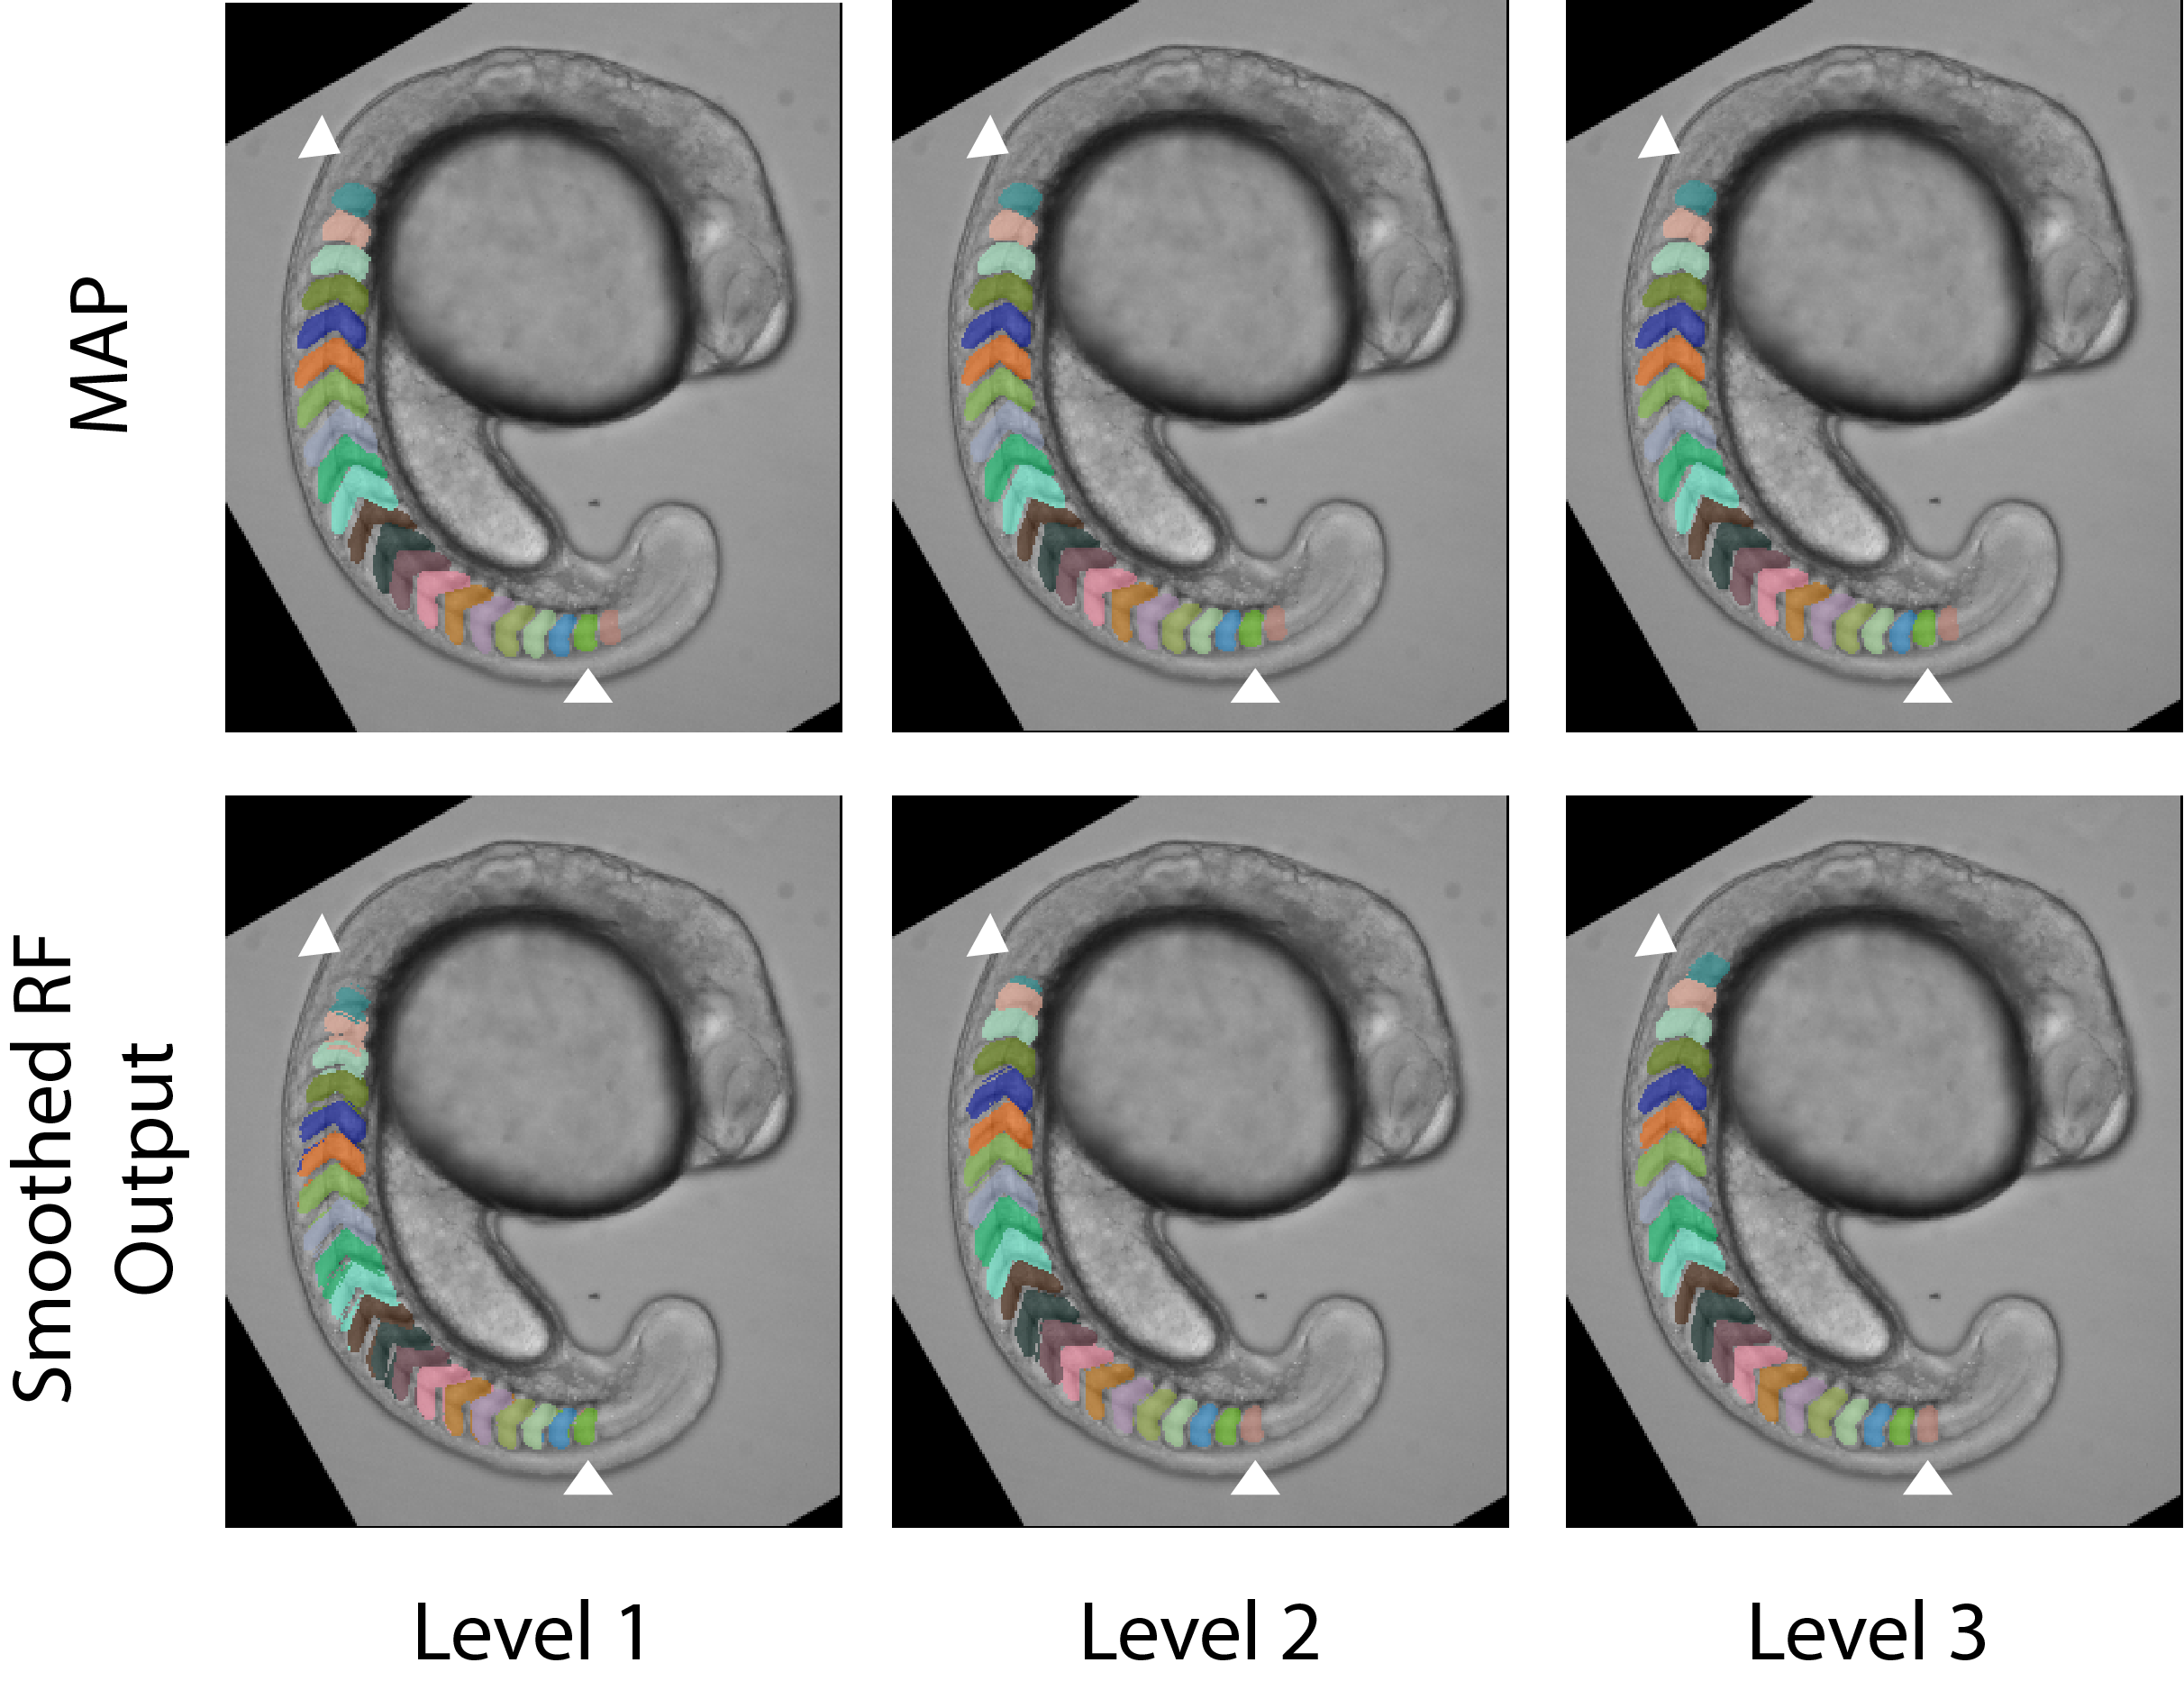
\includegraphics[width=\columnwidth]{rescue.png} %&[trim=0cm 2cm 0cm 1cm,height=0.2\textheight]
\caption{Rescue Case. Arrows point to ground truth start end end of spine. }
\label{fig:rescue}
\end{center}
\end{figure}



{\small
\bibliographystyle{ieee}
\bibliography{somites2014}
}

\end{document}
